\documentclass{article}
\usepackage[utf8]{inputenc}
\usepackage[spanish]{babel}
\usepackage{graphicx}
\usepackage{amsmath}
\usepackage{amssymb}
\usepackage{placeins} 
\usepackage{listings}
\usepackage{vmargin}
\usepackage{hyperref}
\usepackage{multirow}
\usepackage{ulem}
\usepackage{blindtext}
\usepackage[table,xcdraw]{xcolor}
\usepackage{enumitem}
\usepackage{tabularx}
\addtolength{\textwidth}{2cm}
\addtolength{\hoffset}{-1cm}
\setlength\parindent{0pt}
\setlength{\parskip}{0.5cm}
\usepackage[spanish]{babel} % para escribir en espanol
\usepackage{array} % para las tablas
\usepackage{float} % para usar [H]

\title{Parcial Final Arquitectura de Software}
\author{Diana Carolina Muñoz Hurtado \\ Maestría en ingeniería de software }
\date{June 2020}


\begin{document}

\maketitle

\section{Diagramas para la definición arquitectura sistema nacional de reportes covid 19}

\subsection{Diagrama de contexto}

Se inicia con realizar un diagrama de contexto para determinar las fuentes de información indicando cumplir con los 5 objetivos del sistema propuesto:

\begin{figure}[h] 
    \centering
    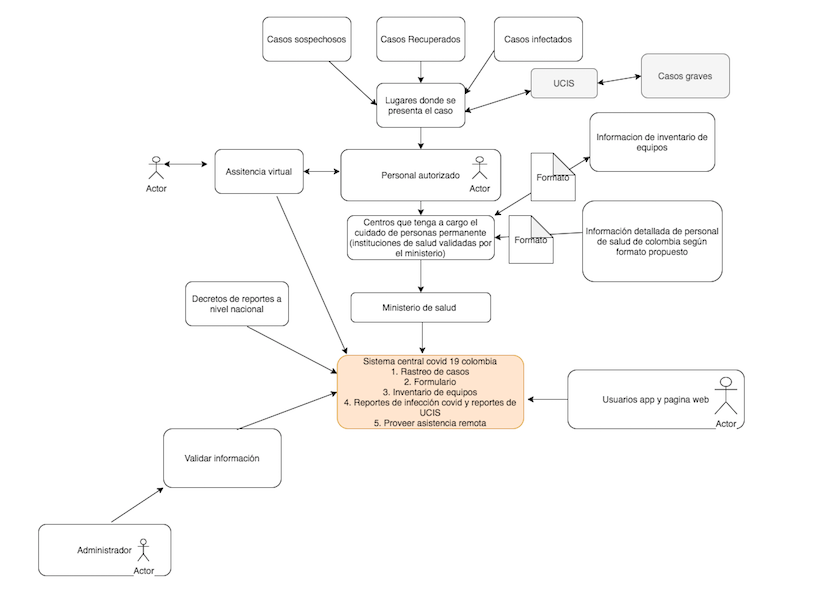
\includegraphics[scale=0.5]{Context.png}
    \caption{Diagrama de contexto sistema nacional de reportes covid 19}
    \label{Arqui}
\end{figure}

\newpage


\subsection{Escenarios de Calidad}

Se definen los siguientes escenarios de calidad para desarrollar la arquitectura teniendo en cuenta que con el diagrama de contexto se determina usar una arquitectura basada en microservicios debido a la variedad de fuentes de información que se necesitan para cumplir los objetivos:

\begin{table}[h]
\begin{tabular}{|
>{\columncolor[HTML]{C0C0C0}}l |l|l|}
\hline
\textbf{Tactica}                                             & \multicolumn{2}{l|}{Almacenamiento de datos con Buckets3 Website}                                                                                                                                                                                                                                  \\ \hline
\textbf{Escenario}                                           & Disponibilidad                                                                                                                                               & Seguridad                                                                                                                                      \\ \hline
Source                                                       & Usuario                                                                                                                                                      & Ataque humano                                                                                                                                  \\ \hline
\textbf{Stimulus}                                            & \begin{tabular}[c]{@{}l@{}}Envio de información: no se esta recibiendo\\ la información requerida por el usuario por \\ la caida de un servicio\end{tabular} & \begin{tabular}[c]{@{}l@{}}Una persona no autorizada ingresa al sistema para \\ asistencia virtual al no tener una clinica cerca\end{tabular}  \\ \hline
Artifact                                                     & Alamacenamiento de datos                                                                                                                                     & Autenticación de usuario                                                                                                                       \\ \hline
Envoriment                                                   & Falla observada en cualquier dia de operación                                                                                                                & En cualquier día de operacíon                                                                                                                  \\ \hline
Response                                                     & Datos alamacenados con capacidad virtual                                                                                                                     & \begin{tabular}[c]{@{}l@{}}Notificar ataque : Sistema de monitereo de salud \\ que necesite autorizacion para acceder a los datos\end{tabular} \\ \hline
\begin{tabular}[c]{@{}l@{}}Response  \\ Mesaure\end{tabular} & 99.99 \%                                                                                                                                                     & \begin{tabular}[c]{@{}l@{}}Los datos correctos se restauran y se identifica \\ la fuente de manipulación\end{tabular}                          \\ \hline
\end{tabular}
\end{table}







\subsection{Arquitectura del sistema}


\begin{figure}[h] 
    \centering
    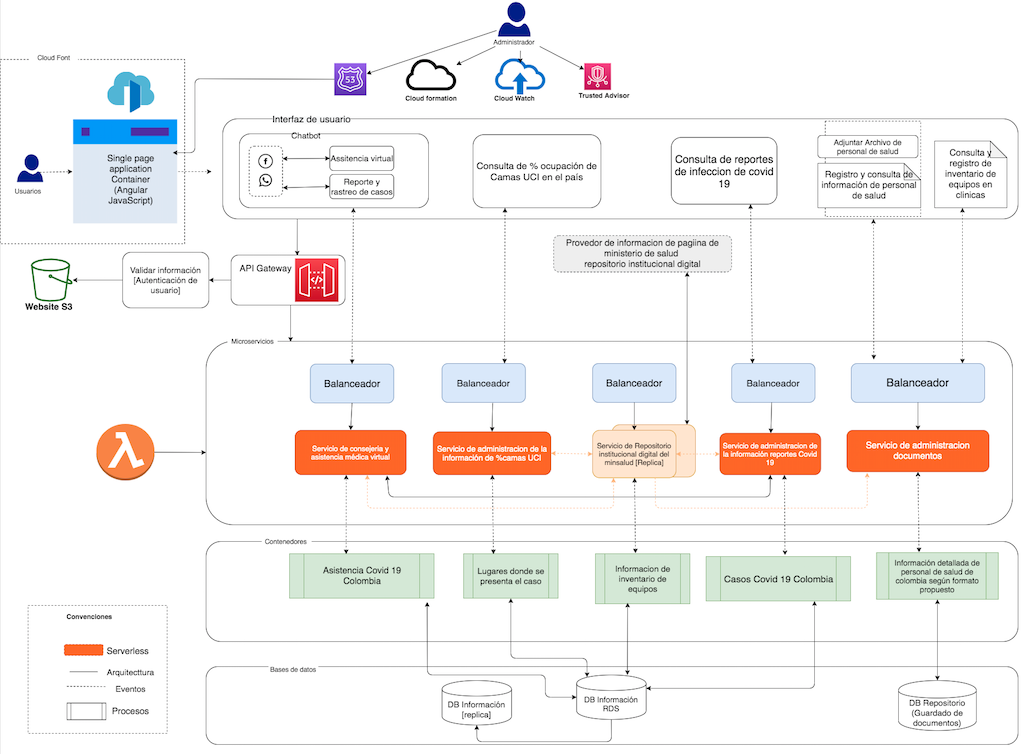
\includegraphics[scale=0.4]{Arquisitem.png}
    \caption{Arquitectura sistema nacional de reportes covid 19}
    \label{Arqui}
\end{figure}

\subsubsection{Explicación de componentes}

\begin{itemize}
    \item \textbf{Interfaz de usuario} cuenta con un chatbot donde a partir de preguntas especificas que el sistema arroje de manera instantánea al usuario se conocerá el estado de salud, cuenta con un campo de asistencia virtual para usuarios que no tienen un centro de salud cercano y que sera llamado en caso de necesitarse, estas preguntas también podrán dar índices de posible caso positivo a Covid 19 y la asistencia virtual también permitirá brindar recomendaciones. Se cuenta con campo para consulta de porcentaje de ocupación de camas UCI, un campo de consulta de reportes de infección  de covid 19, un campo de información para el personal de salud donde podrá adjuntar un archivo, hacer registro o consultar  y por ultimo un campo para consulta y registro de inventarios de equipos de clínicas de cada uno de estos se manejan micro-servicios correspondientes.
    
     \item \textbf{Administrador} Que podrá manejar servicio con diferenetes herramientas la primera para el de nombres de domino (DNS), se usa únicamente con el fin de generar una url amigable para el acceso al sistema de gestión documenta con la utilización del \textbf{Route53:}, el \textbf{Cloudwacth:} Se usa con el fin de generar métrica de uso de los servicios dentro de la arquitectura. \textbf{CloudFormation:} Para brindar la solución de disponibilidad adicional, lo cual permite modelar y aprovisionar, de una manera segura y automatizada, todos los recursos necesarios para las aplicaciones en cualquiera de las regiones. \textbf{Trusted Advisor:} Es una herramienta que permite optimizar los costos de las implementaciones realizadas en Amazon, adicional genera recomendaciones acerca de rendimiento, seguridad y tolerancia a errores.
     
    \item \textbf{Micro-servicios} Se utilizan 5 servicios en el diagrama representados de color naranja que indican que se desarrollan bajo la aplicación serverless, entre ellos se cuenta con un servicio que consulta desde un proveedor información que en este caso es el repositorio institucional digital de minsalud y se analiza la ejecución de una replica de este servicio para proporcionar la disponibilidad de consulta a los demás servicios cuando se requiera en caso de presentar una falla o caída.
    \item \textbf{Contenedores o procesos y bases de datos} Donde se determina la información requerida  por el sistema tal como lo describe el nombre de cada proceso para luego ser almacenado en las respectivas DB RDS y en la DB Repositorio para la documentación del personal.
    
    Se tiene por lo tanto una propuesta de tabla para el registro en base de datos de los documentos con formato solicitado al personal de salud 
    \begin{figure}[h] 
    \centering
    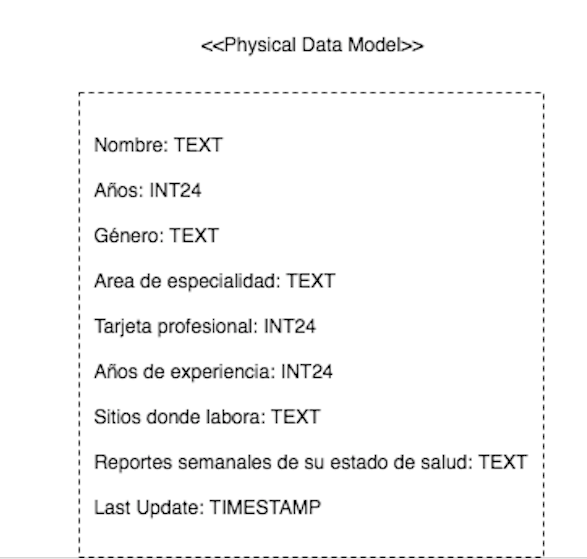
\includegraphics[scale=0.4]{Table.png}
    \caption{Propuesta Tabla de registro de personal de salud}
    \label{Ser}
    \end{figure}



\end{itemize}

Se explica entonces como se desarrolla la aplicación de serverless para los servicios en este caso el de servicio de consejería y asistencia médica y el de administración de información de reportes Covid19, teniendo en cuenta que este a su vez se comunica con el servicio de consulta del repositorio de minsalud para acceder a las recomendaciones nacionales, por lo tanto este se encarga de determinar el estado de salud de la persona con la información que se pueda obtener de las preguntas del chatbot y registra si hay un posible caso covid19:

\begin{figure}[h] 
    \centering
    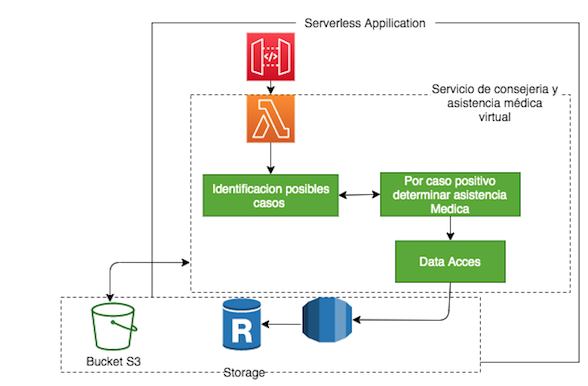
\includegraphics[scale=0.45]{Serverless.png}
    \caption{Aplicación de serverless}
    \label{Ser}
\end{figure}

Debido a que varios de los servicios se comunican con un proveedor de información  ya se puede pensar en las funcionalidades de lectura y comunicación que van en cada de los procesos, como propuesta es usar webscraping para traer información puntual que el usuario desee consultar, Web scraping es una técnica utilizada mediante programas de software para extraer información de sitios web:

\begin{figure}[h] 
    \centering
    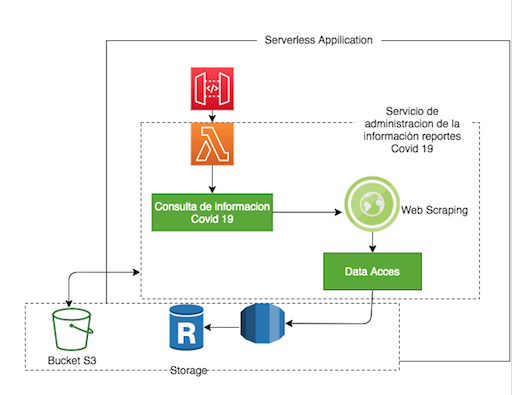
\includegraphics[scale=0.5]{webs.png}
    \caption{Aplicación de serverless y propuesta web scraping}
    \label{Ser}
\end{figure}







\newpage

\susubsection{Decisiones de Arquitectura AWS - serverless}

A medida que se desarrollo el flujo de trabajo se fueron determinado tecnologías necesarias entre las que se tienen:

\begin{itemize}
    \item \textbf{Serverless:} Se opta por una opción serverless debido al potencial de disponibilidad escalamiento de componentes que tiene en AWS, adicional por su velocidad de implementación y puesta a punto de los servicios. \cite{3}
    \item \textbf{Buckets3 Website:} se aloja el sitio web de acceso a usuarios en un bucket debido a su baja latencia y alto nivel de procesamiento, adicional ofrece una durabilidad de 99.999999999\% de los objetos y una disponibilidad de 99.99\% al año.\cite{3}
    
    \item \textbf{Lambda:} Al usar este servicio de Amazon, no se necesita aprovisionar un servidor e instalar los paquetes necesarios que hagan que la aplicación realice las operaciones, al contrario, Amazon lo que ofrece es el enfoque a la funcionalidad del código y no de la configuración, debido a esto al aprovisionar un servicio lambda AWS entrega entre las opciones bajo que motor desea correr el código.\cite{3}
    \item \textbf{RDS DB:} Debido a su alta consistencia, esta base de datos tiene  información fundamental para mantener los flujos de los documentos del personal de salud dentro de la aplicación.
    
    \item \textbf{API gateway:} Una manera efectiva de gestionar los recursos de las diferentes lambdas que contienen los servicios para el manejo de gestión documental es el api Gateway, debido a que es un servicio completamente administrado que facilita la creación, la publicación, el mantenimiento, el monitoreo y la protección de API a cualquier escala
    
   
     
    \item \textbf{Replica RDS:} Se genera una copia de la base de datos RDS con el fin de agregar disponibilidad, debido a que, si por alguna razón la zona donde se encuentra alojada la master de la RDS falla, la replicar  puede suplir los datos. 

    
\end{itemize}




\section{Lectura Architectures Panel}

Una conferencia donde se habla de las diferentes arquitecturas y herramientas que estan impulsando sistemas de software en la actualidad.  Anvita Pandit es una ingeniera de software en Google que menciona cómo crearon el sistema de administración de claves de Google escalable y confiable. Ben Sigelman es CEO y cofundador de LightStep, sobre arquitecturas profundas, cómo escalamos las cosas de manera amplia y qué cosas podríamos hacer en el lado de la observabilidad para que sea sostenible. Justin Ryan de Netflix habla sobre los patrones de escala que Netflix usa en sus servicios de borde. finalmente, Thierry Cruanes de Snowflake habló sobre cómo construir el almacén de datos de Snowflake para aprovechar todas las cosas nuevas que tenemos en la nube. 


Se menciona en esta conferencia el tema de microservicios en organizaciones y como se estan llevando actualmente. por lo general, compañías como Netflix, CircleCI, tienen una aplicación de monolito, por lo que como es su experiencia de dividir algunas funciones en microservicios y también escalarlas en este tipo de sistemas es interesante, por ejemplo, en Netflix,  manejan los clientes de tick o "tick clients". y las migraciones del sistema  que se han realizado se deben a que ya tenían una biblioteca de ticks. Lo que se convierte en una llamada local a una llamada remot invisible para muchos usuarios. esa es una de las razónes por la que se pueden hacer los cambios con el tiempo. En cuanto a cómo se escala, es por que su sistema puede ser escalado horizontalmente.
por lo tanto se abre un debate sobre los sistemas con microsercios y los desafios que trae con su implementacion como problemas de escala. Por lo tanto lo que se propone básicamente es tomar un sistema monolito y ponerlo en marcha en diferentes configuraciones. por lo que para cumplir con la toda la carga de instancias se necesita escalarlas, pero tambien se contrasta la necesidad de implementar microservicios para sistemas o plataformas  que esten inactivos durante 48 horas, entonces es importante aprender de los dominios de cada sistema, entonces se necesita entender tanto el dominio inicialmente, el modelo que se va a construir en micorservicios y las herramientas para hacer la transición de infraestructura; además de ello se mencionan no solo desafíos en software si no en  la forma en que trabajan sus organizaciones de ingeniería o desarrollo. Como parte importante de la construcción de infraestructura en micro-servicios para empresas que quieren hacer una transición es el tema de los proveedores, se habla de un tema de  "diseño basado en dominio" y que el proveedor necesita modelar los datos de la compañía y entender en complejidad cumpliendo con latencia y con-fiabilidad. por lo tanto  se tiene que invertir en las herramientas, la capacitación y las habilidades para poder operar de esa manera. 














\section{Lectura 3 Introducing Dispatch}

En esta publicación Netflix anuncia el lanzamiento de código abierto de marco de orquestación de gestión de crisis para su sistema software: se define entonces Despacho, como : todas las cosas ad-hoc que está haciendo para gestionar incidentes eficazmente  y brindado seguridad mediante una profunda integración con las herramientas existentes utilizadas en toda una organización (Slack, GSuite, Jira, etc.). Dispatch o Despacho  aprovecha la familiaridad existente de estas herramientas para proporcionar la orquestación.
Definiendo tambien, que dispatch se centra especificamente en crear recursos, reunir a los participantes, enviar notificaciones, realizar un seguimiento de las tareas y ayudar con las revisiones posteriores al incidente; lo que te permite concentrarte en solucionar el problema software.  El desafío que se presenta en este caso, es la gestión de incidentes si los mismos incidentes ocurren una y otra vez, por que cada cada incidente es único y extraordinario, por lo que mencionan cuatro componentes principales para la gestión de esta crisis: el primero es la \textbf{gestión de recursos:} la gestión no solo de los datos recopilados sobre el incidente en sí, sino también de todos los metadatos sobre la respuesta.
\textbf{compromiso individual:} comprender la mejor manera de involucrar a individuos y equipos, y hacerlo según el contexto del incidente.
\textbf{gestión del ciclo de vida:} proporciona las herramientas del Comandante de incidentes (IC) para gestionar fácilmente el ciclo de vida del incidente.
\textbf{aprendizaje de incidentes:} a partir de incidentes pasados para acelerar la resolución de incidentes futuros.

Hay bastantes pasos para administrar un incidente y gran parte de esto es manejado de manera ad-hoc. de los cuales se pueden resaltar:

\begin{itemize}
    \item \textbf{Declarar un incidente:} hay muchos puntos de entrada diferentes a un posible incidente: alertas automáticas, una notificación interna o una notificación externa.
    \item \textbf{Determinar el comandante del incidente:} determinar la única persona responsable de conducir un incidente en particular a la resolución en función de la fuente, tipo y prioridad del incidente.
    \item \textbf{Crear canales de comunicación:} La comunicación durante los incidentes es clave.
    \item \textbf{Notificar a las partes interesadas clave:} para cualquier incidente dado, las partes interesadas clave que no participan directamente en la resolución del incidente deben ser informadas del incidente.
\end{itemize}

Aunque esta solucion se desarrolló como una herramienta para ayudar a Netflix a administrar incidentes de seguridad, mencionan que Dispatch tiene como objetivo gestionar todo el ciclo de vida de un incidente, centrándose en involucrar a las personas y proporcionarles el contexto que necesitan para llevar el incidente a la resolución. Por lo que su flujo de trabajo es general que se especifica desde reportar el incidente en el Dispatch UI y  luego se dirije a a una Dispatch API para registrar en una Dispatch DB y de esta API se comunica con las herramientas Slack, JIRA..etc.



 








\section{Bibliografia}

\bibliography{biblio.bib}
\bibliographystyle{IEEEtran}
\nocite{1}
\nocite{2}
\nocite{3}







\end{document}
